\documentclass[a4paper,11pt]{article}
\usepackage[utf8]{inputenc}

% extra packages
% \usepackage{amsrefs}
% \usepackage[autocite=inline,labelalpha=true]{biblatex}

%\usepackage[top=1in, left=1in, right=1in, bottom=1in]{geometry}
\usepackage{geometry}
\usepackage{amsmath, amssymb}
\usepackage{graphicx}
\usepackage{color}
\usepackage{hyperref}
\usepackage{siunitx}

\newcommand{\ve}{\varepsilon}
\newcommand{\h}{\mathcal{H}}

%\setlength{\parindent}{0pt}

\begin{document}
	
	\begin{center}
		\Large \textbf{Research Statement}
		
		\Large Youngmin Park
	\end{center}
	
	
	\section{Introduction}

I develop dimension-reduction methods for neural network models using \textbf{dynamical systems theory}, and in turn, use these findings to understand how biological neural networks function and how they are maintained. I specialize in \textbf{oscillator coupling theory}, \textbf{numerical bifurcation theory}, \textbf{perturbation methods}, \textbf{stochastic dynamical systems}, and \textbf{non-local integro-differential equations}. My independent research program includes the following directions:
\begin{itemize}
	\item \textbf{Coupled oscillators, Section \ref{sec:interactions}}. In summary, I introduced a generalization of coupled oscillator theory, allowing mathematicians to include subtle but important details in reduced phase models that are often neglected by idealized models. This work opens the way for a thorough re-examination of decades of existing oscillator theory that assume either idealized oscillators with strong coupling or general oscillators with weak coupling. There is excellent potential to sharpen questions in problems of diseases such as Parkinsonian tremors. This work is highly compatible with \textbf{Rachel Kuske}'s work on bifurcations in deterministic dynamical systems.
	\item \textbf{Molecular motors, Section \ref{sec:maintenance}}. In summary, I reduced the dimension of a vesicle transport model in confined spaces and analyzed its bifurcations. The model behavior was consistent with experimental observations, suggesting that fluid dynamics forces, molecular motor forces, and the shape of the confinement play significant factors in neural maintenance. This work opens the way for detailed, tractable studies on neural maintenance and how defects in maintenance affect brain function. There is great potential for experimental collaboration. The long-term goal of this work is to help understand the causes and mechanisms behind  brain disorders such as Alzheimer's. This work is highly compatible with \textbf{Rachel Kuske}'s work on stochastic dynamical systems.
	\item \textbf{Cortical network analysis and machine learning, Section \ref{sec:data}}. In summary, I introduced an idealized model of the auditory cortex, which unified disparate optogenetics results in the literature. The model serves as a proof of concept that large numbers of computations in the brain may be handled efficiently by relatively simple neural circuits. This work is an excellent starting point to gain a deeper understanding into the principles underlying general sensory processing. It will lead into the generation of biologically-inspired artificial neural networks which may learn more quickly and robustly than existing methods. This work is highly compatible with \textbf{Leonid Bunimovich}'s work on networks.
\end{itemize}


%I conclude with a comprehensive research plan in Section \ref{sec:research}.

\section{Neural Oscillations}\label{sec:interactions}

%The mammalian neocortex is a key region for numerous functions such as sensory perception and integration, generation of fine motor commands, spatial reasoning, and human language \cite{fuster2002frontal}. Over the past century, researchers have established that the neuron is the computational unit of the cortex, and dense networks of neurons ultimately give rise to complex thought. However, the sheer number and density of connections per cubic spatial unit of cortex poses a daunting scientific challenge. Dimension reduction techniques are invaluable to aid in this endeavor.

%\subsection{Previous Work}

%\textbf{How does the cortex produce patterned activity?} Spatially-modulated neurons such as head direction, place, and grid cells, produce spatio-temporal brain activity that is fundamental to spatial memory and animal survival. The mechanisms underling this activity are not yet well-understood and are difficult to understand from a mathematical and neurobiological perspective. I introduced a method to reduce the dimension of large neural networks, allowing an exploration of the underlying neural mechanisms in great detail. I discovered that interactions between neural adaptation and external inputs contribute to the complex motion of patterned activity in the cortex \cite{park2018scalar}. Only a small set of simple mechanisms can lead to substantial changes in the brain.

%\textbf{How does the cortex control brain rhythms?} In addition to spatio-temporal activity, cortical rhythms are ubiquitous and implicated in behavioral tasks such as attention, memory, and motor coordination. Moreover, large cortical networks produce rhythms that are subject to ever-changing concentrations of neuromodulators. The mechanism of how neuromodulators alter rhythms, and therefore attention, is not well-understood. To better understand this mechanism, I introduced a theory to understand acetylcholine's role in changing the synchronization properties of cortical oscillators. My theory showed that neuromodulators alter the phase response curve (PRC) of neurons and therefore alter the large-scale brain rhythms \cite{park2016weakly}. I extended this result to include strongly asynchronous populations of neurons \cite{park2018multiple}, facilitating future studies of more realistic networks of heterogeneous neurons.

%\textbf{How does the brain process sounds?} The auditory cortex processes sounds in simple but important ways. For example, the auditory cortex adapts to constant background noise by responding less strongly over time, but will respond strongly to sudden changes in the auditory environment. This function is critical to the survival of many animals. To understand how auditory signals are processed, numerous optogenetics labs established differential roles of inhibitory neuron subtypes in processing auditory signals. Labs used different experimental paradigms, so the fundamental role played by each inhibitory subtype was unclear. I unified the experimental results using a single cortical model. The model suggests that numerous brain functions can derive from relatively simple circuits \cite{park2020circuit}.

%
%\begin{itemize}
% \item \textbf{Park, Y.} and Geffen, M.N. \textit{A Mechanistic Model of the Auditory Cortex with Inhibitory Subtypes} (in preparation). We introduce a groundbreaking model of cortical responses to complex auditory stimuli, which includes inhibitory subtypes implicated in such auditory processing. The model readily generates hypotheses for the role of these inhibitory subtypes across multiple experimental results.
%
% \item \textbf{Park, Y.}, Shaw, K.M. Chiel, H.J. Thomas, P.J. \textit{The Infinitesimal Phase Response Curve of Oscillators in Piecewise Smooth Dynamical Systems}. European Journal of Applied Mathematics (2018). We provide a first-principles derivation of the phase response curves (PRCs) of oscillators satisfying non-smooth dynamics. This work is a much-needed extension of the half-century-old theory of PRCs.
% 
% \item \textbf{Park, Y.}, Ermentrout, G.B. \textit{Weakly Coupled Oscillators in a Slowly Varying World}. (2016). We extend the theory of weakly coupled oscillators to account for a slowly varying parameter, greatly facilitating more realistic and topical studies using dynamic parameters. 
%  
% \item \textbf{Park, Y.}, Ermentrout, G.B. \textit{Scalar Reduction of a Neural Field Model with Spike Frequency Adaptation}.
% SIAM Journal on Applied Dynamical Systems (2018). We introduce a novel dimension reduction of so-called ``bump'' solutions of non-local neural field models to centroid coordinates. The dimension reduction allows for a comprehensive analysis of the many bifurcations of the system with greater generality than previously possible.
% 
% \item \textbf{Park, Y.}, Ermentrout, G.B. \textit{A Multiple Timescales Approach to Bridging Spiking- and Population-level Dynamics}. (2018). We introduce a powerful theory that robustly accounts for large frequency differences between populations. This substantial contribution enables computational works to operate without the classic restraint of small frequency differences.
% 
% \item \textbf{Park, Y.}, Heitmann, S., Ermentrout, G.B. \textit{The Utility of Phase Models in Studying Neural Synchronization}. Book chapter in Computational Models of Brain and Behavior. Wiley-Blackwell (2017). In this book chapter, we explore how different types of phase response curves and synaptic connections affect the synchronization properties of a network. This chapter is the first to address this relationship directly, and provides a much-needed guideline for future computational studies.
% 
% \item Shaw, K.M., \textbf{Park, Y.}, Chiel, H.J., Thomas, P.J. \textit{Phase Resetting in an Asymptotically Phaseless System}. SIAM Journal on Applied Dynamical Systems (2012). We derive explicit equations for the phase response curve of a planar, piecewise-linear dynamical system. In contrast to existing beliefs, the work proves that transitions between boundaries can have the greatest effect on the phase response curve.
%
%\end{itemize}
%\subsection{Ongoing Work}

%\cite{ott2008low,kopell2014beyond,nicks2018clusters}
%\cite{golubitsky1986hopf,golubitsky2003symmetry,murza2011oscillation}
%\cite{coombes2001phase,ermentrout2002modeling,coombes2012nonsmooth}

My work on neural oscillations falls within the broader work of oscillator theories oriented towards understanding pathological neural behavior such as Parkinsonian tremors, epilepsy, and cardiac alternans. Overall theoretical work in these directions has been promising, but tend to use one of three starting points: mathematically tractable but very abstract models \cite{ott2008low}, particular forms of symmetry \cite{golubitsky1986hopf}, and the \textit{weak coupling} assumption, or more generally, the \textit{linear} approximation \cite{ermentrout2002modeling}. The weak coupling assumption has long been an invaluable theoretical tool to understand neural behavior consisting of only small deviations from a known behavior such as quiescence or oscillatory activity. Indeed, the weak coupling assumption has driven much of my work \cite{park2016weakly,park2018multiple,park2018scalar}. 

While these assumptions facilitate theorists to a potent degree and were perhaps close to experimental conditions some decades ago, they are now far from modern experimental conditions. Modern experiments are often done \textit{in vivo}, where neurons are often strongly coupled, heterogeneous, and interact nonlinearly. These properties hold in both normal and pathological neural function, so it follows that pathologies can not always be understood using abstraction, symmetry, or linearity. Therefore, my field must develop theories that directly address \textit{strongly coupled} networks of \textit{heterogeneous} neurons with \textit{nonlinear} interactions at multiple scales. We must understand the brain as it is.

To this end, \textit{I have formulated a theory of strongly coupled oscillators} \cite{park2020high}. Consider the coupled system of $N$ ODEs,
\begin{equation}\label{eq:odes}
	\dot X_i = F(X_i) +\ve \sum_{j=1}^N a_{ij} G(X_i,X_j), \quad i=1,\ldots,N,\\
\end{equation}
where each system admits a $T$-periodic limit cycle $Y(t)$ when $\ve=0$. We allow $\ve>0$ not necessarily small and assume general smooth vector fields $F:\mathbb{R}^n \rightarrow \mathbb{R}^n$ and a smooth coupling function $G:\mathbb{R}^n\times\mathbb{R}^n\rightarrow \mathbb{R}^n$. The scalars $a_{ij}$ modulate the strength of coupling between pairs of oscillators, whereas $\ve$ modulates the overall coupling strength of the network.

Let $\theta_i$ be the phase of limit cycle $Y_i$ and define the phase difference $\phi_i=\theta_i-\theta_1$ for $i=2,\ldots,N$. Under general conditions, it is possible to derive a phase reduction of $N-1$ equations,
\begin{align*}
	\dot \phi_i =& \ve\sum_{j=1}^N a_{ij} \h(-\phi_i,\phi_2-\phi_i,\ldots,\phi_N-\phi_i,\phi_j-\phi_i)\\
	&\quad- \ve\sum_{j=1}^N a_{ij} \h(0,\phi_2,\ldots,\phi_N,\phi_j), \quad i=2,\ldots,N,
\end{align*}
where
\begin{equation*}
	\h(\eta_1,\ldots,\eta_N,\xi) = \frac{1}{T} \int_0^T \mathcal{Z}(\eta_1+s,\ldots,\eta_N+s) \cdot G(s,\xi+s)ds,
\end{equation*}
and $\mathcal{Z}$ is the higher-order phase response curve from \cite{wilson2020phase}. My theory produces Taylor truncations of the function $\h$. The higher the truncated order, the more accurately my theory reproduces phase-locked states of $N$ oscillators.

\begin{figure}[ht!]
	\centering
	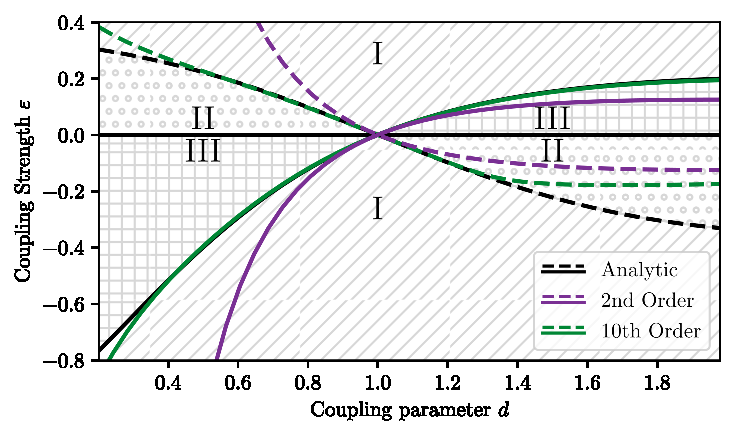
\includegraphics[width=.75\textwidth]{figures/cgl_2par_edited.pdf}
	\caption{Validation of strong coupling theory using diffusively coupled complex Ginzburg-Landau (CGL) models. The plot is a two-parameter bifurcation diagram in coupling parameters $\ve$ and $d$. Synchrony is only stable in regions I and II, whereas antiphase is only stable in regions I and III. Black solid lines denote boundaries where the system switches between stable and unstable synchrony ($\ve_s$). Black dashed lines denote boundaries where the system switches between stable and unstable antiphase ($\ve_a$). Purple solid, dashed: bifurcations detected using 2nd order interaction functions from \cite{wilson2019phase}. Green solid, dashed: bifurcations detected using 10th order interaction functions. \textbf{This result shows that my strong coupling theory substantially outperforms existing coupling theory.}}\label{fig:cgl}
\end{figure}

As a first step, I verified my theory using the mathematically tractable complex Ginzburg-Landau (CGL) model with diffusive coupling. The coupling function has two parameters: $\ve$ for the coupling strength, and $d$ for the degree to which opposing species affect coupling. Both parameters significantly affect the phase-locking properties of the coupled CGL models. I show the accuracy of the theory in the left panel of Fig. \ref{fig:cgl}, where the strong coupling theory (green, tenth-order) coincides strongly with the ground-truth (black) relative to existing coupling theory (purple, second-order) \cite{wilson2019phase}. 

Next, I tested this theory using a realistic four-dimensional model of a thalamic neuron. Figure \ref{fig:thal} shows how my theory predicts phase differences in two thalamic oscillators for different coupling strengths (higher order corresponds to greater accuracy). The right-hand side of the reduced ODE (labeled $-2\h_{\text{odd}}$) is shown in the top row. Roots and slopes correspond to existence and stability of phase-locked states. Phase differences of the full model is shown in the bottom row for 20 difference initial conditions. Coupling strength increases from weak ($g_\text{syn}=0.02$, left column) to strong ($g_\text{syn}=0.25$, right column). \textbf{Roots of the fourth-order reduction coincide with the steady-state phase-locked states of the full system}.

\begin{figure}[ht!]
	\centering
	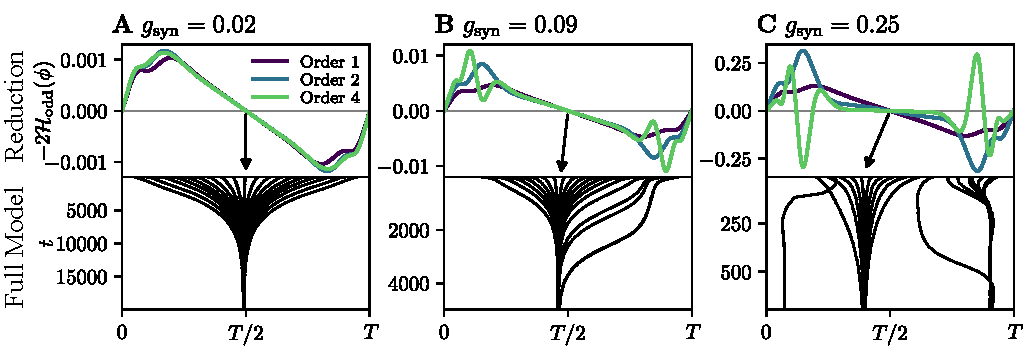
\includegraphics[width=\textwidth]{figures/thal_h_edited.pdf}
	\caption{Performance of the strong coupling reduction compared to a full simulation of thalamic neuron models. A: Weak coupling. The right-hand side of the reduction (top) is shown for different orders (higher is more accurate) and coincides with the long-term phase difference of the full model (bottom). B: Moderate coupling. The reduction (top) coincides with the full model (bottom). C: Strong coupling. The reduction (top) only agrees with the full model (bottom) at order 4. }\label{fig:thal}
\end{figure}

These results demonstrate how my theory is not specific to particular models or coupling functions. Indeed, my theory naturally applies to general coupled oscillator models including those found in physics, biology, and chemistry (the only requirement is that the vector fields of the models are sufficiently smooth).

\subsection{Future Work}

In the long term, I will further develop mathematical methods to analyze neural networks in several important directions. I will augment my theory to include heterogeneity (including n:m phase-locking), making my theory applicable to far more realistic neural networks. I will augment my theory to include oscillator death to understand interactions between bursting neurons in networks such as subcortical networks and central pattern generators. Finally, I will derive the mean-field equations for neural models (in contrast to existing mean-field theories that use idealized models \cite{ott2008low}) to understand how microscopic neural interactions influence large-scale brain activity.

\section{Neural Maintenance: Dendritic Spines} \label{sec:maintenance}

%\cite{kasai2010structural,holtmaat2009experience}
While neural interactions are an important part of understanding how brains function, questions of neural maintenance are equally important. Seemingly minor defects at the nanometer-to-micrometer scale can result in serious disorders at the scale of the whole brain. For example, deficits in molecular motor transport in axons are implicated in neurodegenerative diseases such as Parkinson's disease \cite{millecamps2013axonal}. Another example involves pyramidal neurons, the most ubiquitous type of neurons in the mammalian neocortex. They feature tens of thousands of excitatory convergent synaptic inputs, where most incoming synaptic signals terminate on sub-micron bulbs known as dendritic spines \cite{nimchinsky2002structure}. Spines exhibit a significant degree of morphological plasticity \cite{kasai2010structural} with pathological spine formation implicated in disorders such as Autism spectrum disorder and Alzheimer's disease \cite{penzes2011dendritic}. How spines function and how they are maintained is therefore an important question.

%\cite{park2006plasticity,wang2008myosin}
Dendritic spines receive surface proteins by protein-carrying vesicles that squeeze through the neck of the spine and eventually fuse with the spine head \cite{da2015positioning}. The motion of such vesicles has been observed to not involve only translocation, where the motion is unidirectional, but includes corking, where the vesicle gets ``stuck'' in the spine neck, and rejection, where the vesicle initially enters the spine but eventually reverses direction and exits \cite{park2006plasticity}. \textbf{How molecular motors affect changes in vesicle direction is the goal of ongoing work}.

%\cite{muller2008tug,kunwar2011mechanical}
%\cite{bressloff2009directed,newby2009directed,newby2010random,newby2011asymptotic,bressloff2013metastability}
%\cite{julicher1995cooperative,guerin2011motion,allard2019bidirectional,portet2019deciphering}
Indeed, the importance of this problem has spurred an extensive literature on the effects of molecular motors on vesicle dynamics, including the computation of the distribution of cargo velocities \cite{kunwar2011mechanical}, computing mean first passage times to transport targets on dendritic morphologies \cite{bressloff2013metastability}, and the generation of bidirectional motion despite the assumption of symmetry \cite{portet2019deciphering}. \textit{However, these studies often neglect or fix drag forces which could arise from constriction effects in the unique bulbous shape of dendritic spines}.

To this end, I have reduced a fluid dynamics model of dendritic spine transport into a tractable fast-slow system:
\begin{equation}\label{eq:fs1}
	\begin{split}
		\frac{dZ}{dt} &= U,\\
		\ve\frac{dU}{dt} &= F(U) - \zeta(Z) U.
	\end{split}
\end{equation}
$F$ is the net motor force, $U$ is the vesicle velocity, $Z$ is the vesicle center of mass, and $\zeta$ is the function that captures information about the constriction geometry at position $Z$.

\begin{figure}[ht!]
	\centering
	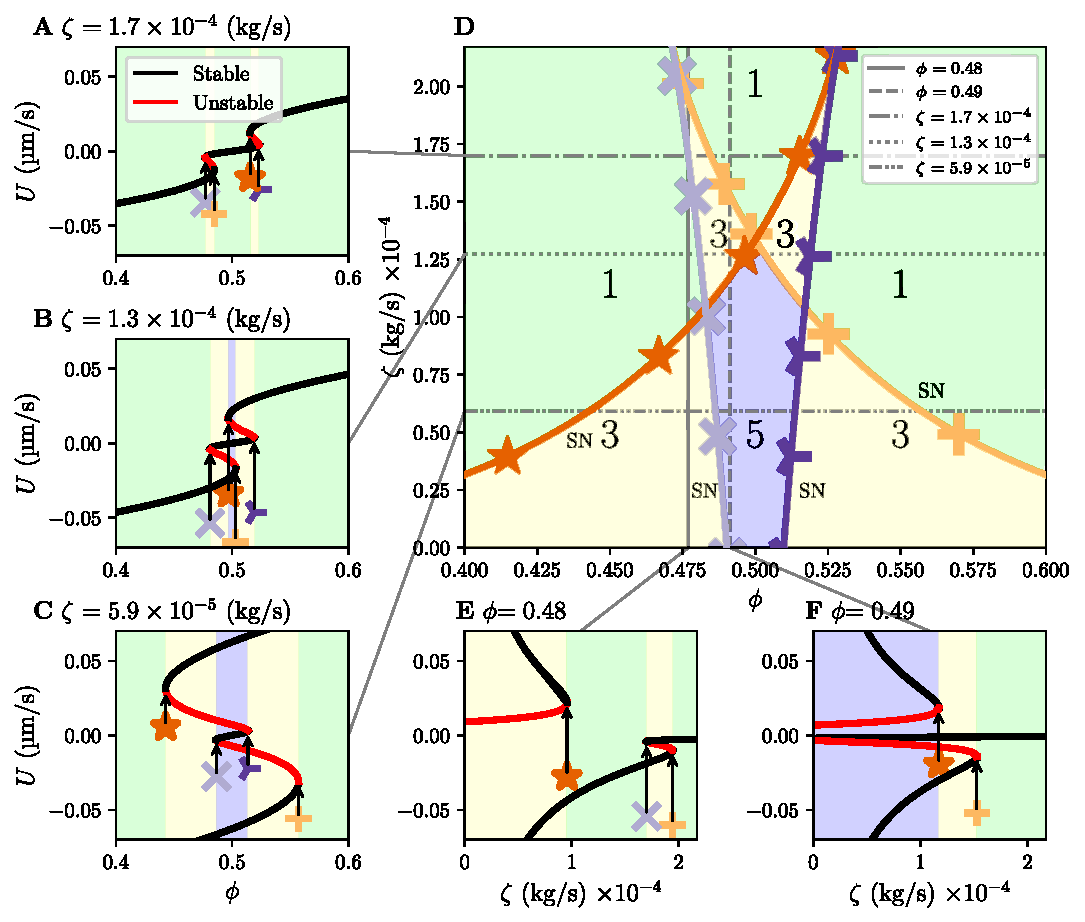
\includegraphics[width=\textwidth]{figures/bifurcations_colored.pdf}
	\caption{Two parameter bifurcation diagram in $\phi$ and $\zeta$. Saddle-node (SN) bifurcations are shown in (D) as colored branches with a unique color and symbol. Numbers in (D) indicate the total number of fixed points in the corresponding region of parameter space. Subplots A, B, C, E, F, show one-parameter slices of the two-parameter diagram. Saddle-nodes are labeled with the corresponding branch color and symbol. The critical vesicle-to-spine diameter ratio at the cusps is roughly 2\si{.\um}/3\si{.\um}.}\label{fig:2par}
\end{figure}

Standard dynamical systems theorems (Fenichel theory) allows us to view the equivalent system in the limit $\ve\rightarrow 0$,
\begin{equation*}
	\frac{dU}{ds} = F(U) - \zeta U,
\end{equation*}
where $\zeta$ is a parameter and  $s=t/\ve$. Using this reduced system, I proved the unique existence of unidirectional motion for sufficiently close vesicle-to-spine diameter ratios. The two-parameter diagram in the confinement factor $\zeta$ and the ratio or up- and down-motors $\phi$ is shown in Figure \ref{fig:2par}. In summary, the two-parameter diagram (panel D) predicts that smaller $\zeta$ (wider constrictions) tend to show bidirectional motion, whereas larger $\zeta$ (tighter constrictions) predict unidirectional motion.

\textit{This result is consistent with experimental observations of vesicle trajectories in the literature \cite{park2020dynamics}}. Experimentally-observed vesicles traveling into thin spines with tight constrictions tend to exhibit unidirectional motion, whereas vesicles traveling into wider, stubby spines tend to exhibit bidirectional motion. The consistency suggests that fluid flow in dendritic spines combined with molecular motor forces contribute significantly to bidirectional vesicle motion. Neurons may modify spines to become wider or thinner depending on the needs of the synapse.

\subsection{Future Work}
While mean-field models are useful with large numbers of agents, sub-micron spines only contain a few dozen myosin motors. \textit{The effects of noise are prominent, and we can not rely on mean-field models to fully understand how spines function}. Thus I will shift my attention to understanding how finite numbers of stochastic motors affect the probability of translocation.

Before turning to the probability of vesicle translocation, I will focus on the specific question of the mean first passage time (MFPT) to switch the direction of vesicle motion. This switching is a well-known ``tug-of-war'' effect \cite{julicher1995cooperative} that has not been studied using myosin motors or with constrictions. I have developed an agent-based simulation where individual myosin motors attach and detach with position-dependent rates in order to compute MFPTs. However, agent-based simulations are computationally expensive: to obtain mean first passage times (MFPT), roughly 5-10 trials must be run in parallel over 50-100 time units with time steps on the order of 1e-6. These requirements mean dozens of hours per simulation. I will overcome the problem of long simulation times through the use of a master equation approximation.


%The Fokker-Planck equation and corresponding Langevin equation would have been ideal, but they fail to work for our system, which is a class of birth-death models \cite{doering2005extinction}. I have therefore turned to the master equation, which presents its own set of challenges. In existing literature, molecular motors typically do not have spatial dynamics, and have position-independent attachment and detachment rates. A master equation formulation is therefore very straightforward to derive. In contrast, the myosin motor depends on position and velocity, which affect the detachment rates in a way that standard steady-state assumptions are not valid. To account for the dependencies, I included the appropriate position and velocity dependencies into a modified version of the master equation. Some problems remain to be ironed out, but this master equation largely reproduces the MFPT of the agent-based model with a speed improvement in two orders of magnitude.

%I will turn to the question of how constrictions affect the probability of vesicle translocation and compute the mean first passage time of vesicle translocation. Due to the increasing complexity of the model, I may turn to additional simplifying assumptions and further abstract the model to make this question tractable. The future directions beyond this point are plentiful. For example, protein-carrying vesicles serve as part of a greater maintenance complex that includes maintaining the receptor density, modifying the spine shape and size, and increasing the reliability of postsynaptic spine responses. I will pursue questions on how translocation affects the function of the greater complex, and how the spine maintains an optimal shape for a given function.

%\section{Research Plan}\label{sec:research}

%The long-term goal of my research is twofold. First, to further develop new dimension reduction strategies that can be used to understand neural interactions and neural maintenance, and second, to combine the research insights from my work to build a comprehensive understanding of brain function. In my future research, I will research how the maintenance of individual spines affect the neural response properties of synapses distributed throughout neurons and networks. This work naturally relates to understanding how changes in dendritic spines affect the communication of neurons in brain networks, and leads to a holistic understanding of how neural dysfunction affect disorders such as Alzheimer's and autism.

%My overall research is mathematical, computational, and biological. It provides ample opportunities for students at any level to engage in state-of-the-art multidisciplinary research. Preferred backgrounds include (but are not limited to ) mathematics, biology, computer science, physics, and chemistry. Because my work is at the intersection of many fields, my students will learn to communicate with people of diverse backgrounds, and will learn general methods in mathematics and programming.

\section{Cortical Network Analysis and Machine Learning}\label{sec:data}

I introduced an idealized model of the auditory cortex unifying numerous experimental results in the field of auditory neuroscience \cite{park2020circuit}. This model demonstrated that simple cortical mechanisms including synaptic facilitation and depression are sufficient to reproduce numerous types of auditory processing. The model included excitatory (pyramidal) neurons as well as the inhibitory subtypes somatostatin-positive (SOM) and parvalbumin-positive (PV) interneurons, which were necessary to reproduce optogenetic results. Many questions remain regarding robustness of the model and its similarity to real cortical networks. While we performed some parameter sweeps, the ability of the model to reproduce additional auditory phenomena was not explored in depth.

In addition, I worked with a neuroscientist who ran auditory experiments on mice. They generated many gigabytes of partially-observed calcium traces, which were generated as the mouse responded to auditory tasks. In order to generate correlations between all observed neurons, I used subspace identification to recover correlations when pairs of neurons were not observed on a given trial. The method included the use of stochastic gradient descent to estimate the optimal correlation matrix corresponding to the partial data. Once this was performed, I used hierarchical clustering and found that correlated neurons tended to be spatially clustered in the cortex (unpublished).

\subsection{Future Work}
Machine learning is an incredibly powerful, general tool, yet learning algorithms then to be extremely expensive in terms of trials, requiring countless iterations. In contrast, animals tend to learn with far fewer iterations. I hypothesize that there exist neural networks with biologically-inspired constraints that are capable of learning far more rapidly than a general neural network.

To this end, I will view the cortex as a large number of coupled differential equations with heterogeneous parameters. This starting point is natural from a modeling perspective because all parameters and connections are explicit. It is also general, extending beyond cortical responses to auditory inputs, indicating just how powerful this framework can be. My goal is to use automated and theoretical tools, including machine learning and inverse methods, to uncover the parameter spaces within which healthy and unhealthy cortical networks operate. This information will include connectome data as well as connectivity data in dendrites and axons in order to uncover which aspects of the physical organization in the cortex contribute most to network performance. This information will in turn better constrain artificial neural networks and improve performance \cite{lee2018training}.


\bibliographystyle{plain}
\bibliography{refs.bib,../youngmin-bard/bio,../youngmin-bard/neuralfield,../youngmin-bard/math,../youngmin-bard/phase,../youngmin-bard/computation,../youngmin-bard/cortex,../thomas-youngmin/notes/spines.bib,../thomas-youngmin/notes/vesicles.bib,../thomas-youngmin/notes/noise.bib,../thomas-youngmin/notes/motors.bib}


\end{document}
